\documentclass[12pt]{article}

\usepackage[utf8]{inputenc}
\usepackage[brazilian]{babel}
\usepackage{graphicx,url}
\usepackage{sbc-template}
\usepackage{mermaid}
\usepackage{comment}

\urlstyle{same}

\sloppy

\title{Mineração de Microdados do ENEM para Identificação de Escolas com Bom Desempenho em TIC em Contextos Socioeconômicos Desfavoráveis}

\author{Felipe Lacerda Tertuliano\inst{1}, Maria Inês Martins\inst{1}}

\address{Pontifícia Universidade Católica de Minas Gerais (PUC Minas)\\30.535-901 - Belo Horizonte - MG - Brazil}

\begin{document}

\maketitle

\begin{abstract}

This work proposes the development of an analytical mechanism to identify schools in the public basic education network as targets for training interventions in Information and Communication Technologies (ICT). Using microdata from ENEM and the School Census, the methodology involves large-scale data analysis that combines student performance in the national exam with socioeconomic indicators and school characteristics. The objective is to identify institutions with performance that deviates from expectations, thereby directing public policies and resources more effectively. This will result in a prototype, such as reproducible scripts or a panel of indicators, which will contribute to applied data science, education, and training in ICT in Brazil.

\end{abstract}

\begin{resumo}

Este trabalho propõe o desenvolvimento de um mecanismo analítico para identificar escolas da rede pública de ensino básico como alvo para intervenções em capacitação em Tecnologias da Informação e Comunicação (TIC). Utilizando microdados do ENEM e do Censo Escolar, a metodologia envolve a análise de dados em larga escala, cruzando o desempenho dos estudantes no exame nacional com indicadores socioeconômicos e características das escolas. O objetivo é identificar instituições com desempenho que fogem ao esperado para direcionar políticas públicas e recursos de forma mais eficaz, resultando em um protótipo, como scripts reprodutíveis ou um painel de indicadores, contribuindo para a ciência de dados aplicada à educação e à formação em TIC no Brasil.

\end{resumo}

\section{Introdução}

A educação é o principal pilar para o desenvolvimento de qualquer área técnica, especialmente no processo de capacitação em que as condições materiais e sociais como a renda, ambiente de estudo, etnia ou gênero podem afetar as oportunidades e o desenvolvimento desses futuros profissionais. No Brasil a desigualdade social, a violência, baixos investimentos e vários outros fatores (característicos de países em desenvolvimento) afetam diretamente o processo de escolarização. Ainda assim, em condições desfavorável há casos escolares de sucesso, os quais são, entretanto, de difícil identificação e compreensão. Quais e como essas exceções geraram esses resultados? Esse trabalho tem como objetivo o desenvolvimento de um mecanismo analítico para identificar escolas-alvo para intervenções de capacitação em Tecnologias da Informação e Comunicação (TIC) para alunos da rede pública de ensino básico. O mecanismo de identificação se pautará em dados públicos, sobretudo no cruzamento de de informações extraídas dos microdados do Exame Nacional do Ensino Médio (ENEM) e dos microdados do Censo Escolar, ambos disponibilizados anualmente pelo Instituto Nacional de Estudos e Pesquisas Educacionais Anísio Teixeira (INEP).

Partindo do pressuposto de que o desempenho educacional em competências digitais depende, para além da infraestrutura tecnológica disponível, de fatores pedagógicos e institucionais, podemos identificá-los por meio da análise de dados educacionais em larga escala. Nesse contexto, a construção de um sistema de análise orientado por dados pode contribuir para orientar políticas públicas de formação e apoio às escolas, especialmente em contextos socioeconômicos mais vulneráveis. Os microdados contêm informações detalhadas sobre o desempenho dos participantes nas diferentes áreas do exame, variáveis relacionadas ao perfil socioeconômico dos estudantes e dados das escolas.

A proposta consiste em extrair, tratar e organizar esses dados utilizando técnicas de tratamento de grandes bases de dados, análise estatística e de agrupamento, possibilitando a construção de indicadores comparáveis entre escolas. A análise privilegiará o cruzamento entre três conjuntos de variáveis: 1. o desempenho dos estudantes em competências associadas ao uso e à compreensão de Tecnologias da Informação e Comunicação, 2. os indicadores socioeconômicos declarados pelos participantes no questionário contextual do ENEM e 3. As características específicas da instituição de ensino em que esse participante se formou. Para o desempenho, serão consideradas competências presentes na Matriz de Referência (MR) do ENEM da área de Linguagens, Códigos e suas Tecnologias (C1 e C9) e na MR de Matemática e suas Tecnologias (C7), por estarem relacionadas a habilidades de interpretação de informações, resolução de problemas e uso de recursos tecnológicos e informacionais. Os indicadores socioeconômicos permitirão, de outro lado, caracterizar o perfil dos estudantes e/ou da escola e construir índices sintéticos ou classificações que representem as instituições. O cruzamento entre desempenho nas competências selecionadas e a situação das escolas permitirá identificar padrões de desempenho que escapam às expectativas associadas às condições SE e, se possível, infraestruturais.

A identificação dessas unidades escolares, com desempenho resiliente, permitirá orientar ações de capacitação em TIC baseadas em evidências, direcionando recursos e estratégias para contextos em que tais intervenções possam produzir maior impacto. Como produto final, pretende-se desenvolver um protótipo de mecanismo de identificação de escolas-alvo, que poderá assumir a forma de um conjunto de rotinas de análise de dados, scripts reprodutíveis ou mesmo um painel analítico que permita visualizar e comparar indicadores educacionais e socioeconômicos. Espera-se que a proposta contribua tanto para o campo da ciência de dados aplicada à educação quanto para o aprimoramento de estratégias de formação em TIC no sistema educacional brasileiro.

\section{Revisão de Literatura}

O Exame Nacional do Ensino Médio (ENEM) foi criado em 1998 no Brasil com o intuito de avaliar a educação na rede de escolas do ensino médio nacionais. A adesão ao ENEM foi tímida nas primeiras edições do exame, mas ganhou força, a partir da edição de 2004, quando passou a ser o mecanismo de ingresso ao Programa Universidade para Todos (ProUni), com disputa nacional de bolsas de estudo em instituições privadas. O exame era feito em uma única tarde, composto por uma prova com 63 questões objetivas e uma redação. A sua consagração ocorre, a partir da sua edição de 2009, em que foi reestruturado para o modelo conhecido atualmente, e passou a ser também o mecanismo de ingresso ao Sistema de Seleção Unificada (Sisu). O exame passou a ser feito em 2 turnos, composto por uma redação e quatro provas de 45 questões cada uma, agrupadas por área de conhecimento, a saber: Códigos, Linguagens e suas Tecnologias, Matemática e suas Tecnologias, Ciências da Natureza e suas Tecnologias e, Ciências Humanas e suas Tecnologias. O ENEM representa, na atualidade, a principal forma de democratização do ensino superior, configurando-se também como métrica para se avaliar o Ensino Médio, a etapa final da educação básica \cite{misc:decreto_enem} e prognosticar tendências na educação no país, como base concreta para o desenvolvimento de políticas públicas.

Entre outras ferramentas relevantes para o diagnóstico e o desenvolvimento da educação brasileira temos o Censo Escolar, coordenado pelo Instituto Nacional de Estudos e Pesquisas Educacionais Anísio Teixeira (Inep), o que permite o aprofundamento ainda maior na análise sobre ensino Brasileiro. O Censo é preenchido anualmente e com caráter declarativo obrigatório para as escolas da educação básica o censo provê dados da estrutura dessas instituições que também servem de métrica para ações no país. Tanto as informações do ENEM como do Censo Escolar são disponibilizadas em seu estado bruto, através de microdados, os quais se configuram como nossas principais fontes de dados.

Entretanto, somente a disponibilidade desses dados \cite{misc:micro_enem} \cite{misc:micro_escolas} não permite um entendimento concreto sobre a educação, nem possibilita traçar uma abordagem compatível com a realidade do Brasil. Em "Influência da Renda no Desempenho dos Estudantes no Enem: uma Análise Longitudinal" \cite{article:renda_enem}, que fez uma análise de todas as edições do ENEM até 2023 cruzando os dados do questionário socioeconômico com as notas do exame, foi avaliado que, durante todos os anos, a renda familiar foi um fator decisivo para o desempenho dos alunos. Os autores também é destacam a importância da ação direcionada para as escolas públicas e em situação desfavorável, pois são nessas escolas em que se encontram os estudantes mais afetados pela desigualdade social.

Especificamente quando se discute o desempenho nas áreas do conhecimento, disparidades mais complexas podem aparecer, como em "\textit{The Analysis of Mathematics Performance in the National High School Exam in Brazil}" \cite{article:mat_enem}, em que se analisa o desempenho dos candidatos nos testes de matemática do ENEM 2022 com recortes geográficos e de gênero. Nele se mostrou que mulheres, em todos os casos, tinham piores resultados nessa área do exame, o que pode significar uma deficiência no nosso sistema educacional sobre o ensino de exatas.

Assim, a proposta do desenvolvimento de uma ferramenta capaz de mapear esses fatores e identificar pontos de atenção se mostra uma solução não apenas possível, mas também necessária. Na dissertação "Análise dos microdados do Enade: proposta de uma ferramenta de exploração utilizando mineração de dados" \cite{mastersthesis:md_enade} utilizando metodologias de mineração e \textit{machine learning} foi construída uma ferramenta \textit{web} de análise. Entre os achados à partir dos dados foi possível gerar regras que representam condições de alunos no ensino superior, o que é uma forte ferramenta para intervenções direcionadas.

\begin{comment}

Para um melhor entendimento do problema e análise de possíveis soluções foram analisados alguns trabalhos correlatos. 

\subsection{What does the National High School Exam (ENEM) tell Brazilian society?}

\textit{What does the National High School Exam (ENEM) tell Brazilian society?} \cite{article:a_enem} analisa o exame do ENEM e o censo escolar no contexto de 2009 e 2010 para avaliar o impacto e eficiência do exame no Brasil. A partir do trabalho foi possível concluir que condições socioeconômicas explicavam a maior parte das diferenças de notas por escolas, e que pode ser injusta a avaliação dessas instituições por medias brutas, devido ao contexto. Um problema encontrado foi a amostragem, devido ao ENEM ser voluntário não é possível ter uma visão completa da situação da educação no país.

\subsection{Socioeconomic Analysis of students who took the Enem between 2019 and 2022 using Machine Learning}

Em \textit{Socioeconomic Analysis of students who took the Enem between 2019 and 2022 using Machine Learning} \cite{article:se_ml_enem} baseado nos testes do ENEM dos anos de 2019 até 2022 foi aplicado algoritmos de \textit{machine learning} para traçar grupos e características que correlacionarem os resultados da prova com as condições socioeconômicas (SEs) dos participantes. Os resultados formaram dois grupos: alunos mal e bem sucedidos no exame, esses com correlação direta ao seu contexto SE, o que confirma a relevância desses indicadores para nosso objetivo. Entretanto foi observado que o numero reduzido de grupos pode ser um fator que limita conclusões mais profundas sobre possíveis intervenções, junto disso dado que a correlação entre o questionário SE e os resultados das provas foi removido para o ano de 2024, nossa metodologia deve considerar outras formas de extrair informações equivalentes.

\subsection{Impact of Knowledge of Natural Sciences on ENEM Performance: Considerations about Scientific and Technological Inequality to Social Justice}

No artigo \textit{Impact of Knowledge of Natural Sciences on ENEM Performance: Considerations about Scientific and Technological Inequality to Social Justice} \cite{article:nc_enem} avalia o desempenho dos alunos na área das ciências naturais da prova do ENEM de 2017 e como esses resultados são afetados pela estrutura das escolas em que esses estudaram (rede de ensino e presença de laboratório de ciências). Os resultados mostram uma grande diferença na nota de alunos da rede publica e privada, onde mais da metade dos primeiros não alcançou 600 pontos, o que contrasta com o segundo grupo que teve um resultado oposto. A análise dos dados do ENEM por área de conhecimento junto do das escolas mostra uma importante forma de obter grupos e indicadores relevantes para o objetivo do trabalho.

\subsection{Understanding a Profile of the Participants of the Exame Nacional do Ensino Médio (ENEM), Brazil, in the Year 2019, Through Data Analysis}

\textit{Understanding a Profile of the Participants of the Exame Nacional do Ensino Médio (ENEM), Brazil, in the Year 2019, Through Data Analysis} \cite{article:p_da_enem} analisa dentro da base de dados dos participantes do ENEM 2019 fatores que podem influenciar os resultados na prova. Utilizando de algoritmos de análise de dados foi possível traçar relação direta entre condições socioeconômicas e as notas, igualmente para grupo étnico. Mesmo que para os dados do ENEM 2024 não seja possível mais fazer essa relação ainda o estudo é uma base para formas de tratar os dados e direcionar a perspectiva da análise.

\subsection{Análise dos microdados do Enade: proposta de uma ferramenta de exploração utilizando mineração de dados}

A dissertação \textit{Análise dos microdados do Enade: proposta de uma ferramenta de exploração utilizando mineração de dados} \cite{mastersthesis:md_enade} utiliza da base de dados do Enade e metodologias de mineração e \textit{machine learning} para construir uma ferramenta \textit{web} de análise. Entre os achados da mineração foi possível gerar regras que representam condições de alunos dentro do ensino superior, o que pode ser uma forma de identifica públicos alvo. No geral a metodologia da dissertação pode ser utilizada como referencia para atingir resultados com mais qualidade.

\subsection{Clusters de Unidades Federativas do Brasil segundo características socioeconômicas e educacionais dos inscritos no Enem 2021}

A dissertação \textit{Clusters de Unidades Federativas do Brasil, segundo características socioeconômicas e educacionais dos inscritos no Enem 2021} \cite{mastersthesis:c_uf_enem} aplica técnicas de Análise de Agrupamentos (hierárquicas e k-means) aos microdados do Enem 2021 para investigar agrupamentos das Unidades Federativas (UFs) brasileiras. Com variáveis como instrução dos pais, ocupação da mãe e proporção de autodeclarados pretos, pardos ou indígenas, o estudo identifica clusters em algumas regiões geográficas, além de UFs isoladas (Ceará, Distrito Federal e Roraima). Os resultados mostram um cluster distinto formado por Rio de Janeiro e São Paulo, assim como pelos estados da região sul (Paraná, Santa Catarina e Rio Grande do Sul). Este trabalho é relevante para o presente estudo por demonstrar como a Análise de Agrupamentos pode ser aplicada aos dados do Enem para identificar padrões socioeconômicos e educacionais, servindo como referência metodológica para construir indicadores comparáveis entre escolas e identificar instituições com desempenho resiliente.

\subsection{Fatores e evidências sobre o Exame Nacional do Ensino Médio (Enem): uma abordagem exploratória e experimental com mineração de dados}

O estudo \cite{mastersthesis:f_enem} analisa os microdados do Enem de 1998 a 2019 por meio de algoritmos de seleção de atributos e classificadores, identificando que um conjunto reduzido de 10 fatores é capaz de classificar o desempenho estudantil com precisão média superior a 80\%. Os resultados indicam que o tipo de escola cursada no Ensino Fundamental, a renda familiar, a escolaridade materna e a língua estrangeira escolhida estão entre os fatores mais preditivos. A pesquisa evidencia que a dimensionalidade dos dados pode ser reduzida sem perda significativa de acurácia, facilitando análises educacionais direcionadas.

\subsection{Ensaios sobre o Desempenho dos Estudantes no ENEM 2017}

A tese \cite{phdthesis:e_enem} analisa o desempenho de concluintes do ensino médio no ENEM 2017, abordando três fatores principais. O primeiro ensaio investiga a influência direta e indireta da escolaridade dos pais, mostrando que o controle por variáveis como renda e escola reduz significativamente o efeito bruto da educação parental, restando um efeito líquido entre 1\% e 7\%. O segundo ensaio utiliza decomposição quantílica para comparar escolas públicas e privadas, revelando que o diferencial de desempenho é explicado majoritariamente pelo efeito composição (background socioeconômico da turma e da família), enquanto o efeito estrutural é mais relevante nos quantis inferiores. O terceiro ensaio investiga a similaridade de gênero e raça entre professor e aluno, concluindo que alunas se beneficiam de professoras mulheres em Redação e Matemática, e alunos pretos/pardos se beneficiam de professores de Matemática da mesma raça, contribuindo para a redução do gap educacional.

\subsection{Mineração em dados do ENEM para a predição do desempenho acadêmico no âmbito da Rede Federal de Educação Tecnológica}

Nessa dissertação \cite{mastersthesis:md_enem} se aplicou técnicas de mineração de dados sobre os microdados do ENEM 2014 para classificar o desempenho acadêmico de alunos provenientes da Rede Federal de Educação Tecnológica. Foram utilizados seis algoritmos de aprendizado de máquina (JRIP, PART, J48, Random Forest, Naive Bayes e SVM) em uma base pré-processada de 23.354 registros. Os experimentos demonstraram que os modelos Random Forest e Naive Bayes alcançaram as melhores métricas, com acurácia média de 74,32\% e área sob a curva ROC de 0,817. O estudo também extraiu regras de classificação interpretáveis capazes de auxiliar gestores educacionais na identificação precoce de alunos com risco de baixo desempenho no exame.

\subsection{Influência do acesso à internet e ao computador na proficiência de estudantes de baixa renda: uma análise com os participantes do ENEM entre 2015 e 2023}

O estudo apresentado \cite{mastersthesis:i_t_enem} investiga o impacto do acesso domiciliar à internet e ao computador no desempenho de estudantes de baixa renda no ENEM, utilizando uma amostra de 1,5 milhão de alunos entre 2015 e 2023. Por meio de modelos de regressão e técnicas de machine learning, a autora demonstra que o acesso combinado a ambos os recursos produz efeito significativo na proficiência, especialmente durante e após a pandemia de COVID-19, enquanto o acesso apenas à internet, predominantemente via dispositivos móveis, apresenta impacto positivo, porém modesto. O trabalho também evidencia desigualdades de gênero e regionais, reforçando a necessidade de políticas públicas alinhadas ao ODS 4.

\end{comment}

\section{Metodologia}

Para o objetivo do projeto foram escolhidas duas bases de dados a serem tratadas: microdados do ENEM 2024 \cite{misc:micro_enem} e microdados do censo escolar 2024 \cite{misc:micro_escolas}. A partir dessas bases foi iniciada a produção de uma ferramenta na linguagem de programação \textit{Rust} \cite{misc:rust_lang} que seja capaz de ler os microdados, tratá-los e processá-los, gerando enfim indicadores relevantes para a proposta. Um repositório \cite{misc:proj_repo} no \textit{GitHub} \cite{misc:github_repo} foi criado para o versionamento e foi escolhida a \textit{IDE VSCode} \cite{misc:vscode_ide} para o desenvolvimento. Entendendo que o projeto desenvolvido está sujeito a mudanças e possíveis extensões à depender de futuras pesquisas, optou-se pelo uso da arquitetura em N camadas \cite{book:n_layers} seguindo os princípios \textit{SOLID} \cite{misc:solid} de desenvolvimento.

Para guiar a metodologia foi utilizado o processo \textit{Knowledge Discovery in Databases} (KDD) \cite{article:kdd}, no qual se divide a mineração dos dados em etapas, cada uma com um objetivo a fim de melhorar a transformação de dados em informação, conhecimento e, enfim, em ação. Essa sessão será dividida em cinco subseções, cada uma representando e desenvolvendo uma parte do processo KDD, a saber: 1. Seleção, 2. Pre-processamento, 3. Transformação, 4. Mineração e 5. Interpretação.

\begin{figure}[htbp]
\centering
\begin{mermaid}
flowchart LR
  D1@{ shape: cyl, label: "Dados" }
  P1@{ shape: rect, label: "#1 Seleção" }
  D2@{ shape: lin-cyl, label: "Dados\nSelecionados" }
  P2@{ shape: rect, label: "#2 Pre-processamento" }
  D3@{ shape: docs, label: "Dados\nPre-processados" }
  P3@{ shape: rect, label: "#3 Transformação" }
  D4@{ shape: docs, label: "Dados\nTransformados" }
  P4@{ shape: rect, label: "#4 Mineração" }
  D5@{ shape: doc, label: "Padrões" }
  P5@{ shape: rect, label: "#5 Interpretação" }
  D6@{ shape: tri, label: "Conhecimentos" }

  D1 --> P1 --> D2 --> P2 --> D3 --> P3 --> D4 --> P4 --> D5 --> P5 --> D6

  classDef p fill:#7BA7D0,stroke:#4A7AA9,color:#1a1a1a,stroke-width:1px
  classDef d1 fill:#D98F8F,stroke:#B56565,color:#1a1a1a,stroke-width:1px
  classDef d2 fill:#CD9F7A,stroke:#A87D5A,color:#1a1a1a,stroke-width:1px
  classDef d3 fill:#BDB06F,stroke:#978D4F,color:#1a1a1a,stroke-width:1px
  classDef d4 fill:#A4BA6B,stroke:#7E944B,color:#1a1a1a,stroke-width:1px
  classDef d5 fill:#8DC07A,stroke:#6A9657,color:#1a1a1a,stroke-width:1px
  classDef d6 fill:#7CC08C,stroke:#559662,color:#1a1a1a,stroke-width:1px

  class P1,P2,P3,P4,P5 p
  class D1 d1
  class D2 d2
  class D3 d3
  class D4 d4
  class D5 d5
  class D6 d6
\end{mermaid}
\caption{Diagrama baseado no processo KDD \cite{article:kdd}}
\label{fig:kdd}
\end{figure}


\subsection{Seleção}

As bases dos resultados do ENEM quanto do Censo Escolar são obtidas a partir de um \textit{link} na \textit{internet} que permite o acesso livre à um arquivo \textit{.zip} no qual se encontra um conjunto de elementos e, como foco para o projeto, um documento \textit{.csv} contendo os dados. Seguindo o princípio de subsunção de Liskov (SOLID) foi projetado um elemento pai chamado \textit{DataSource} que permite herança de suas funcionalidades para diferentes fontes e dois filhos representando cada uma das bases alvo.

Dentre as funcionalidades implementadas foi criado um fluxo de extração dos dados em três etapas, a saber: 1. Busca-se em um cliente \textit{HTTP} o arquivo compactado das fontes, 2. Descompacta-se e salvo-se o arquivo em um diretório local e 3. O documento \textit{.csv} é acessado utilizando de um caminho pré-definido pelo usuário. Após o acesso a planilha, lê-se linha à linha e as colunas e seus respectivos valores são identificados e finalmente entram na parte de filtragem.

Seguindo a proposta de trabalho para os resultados do EMEM é necessário avaliar quais dos participantes não faltaram ou foram eliminados das provas de Linguagens e Códigos e Matemática (áreas correlacionadas com a capacitação em TIC).Para isso foram removidos todos os elementos em que os campos "TP\_PRESENCA\_LC" e "TP\_PRESENCA\_MT" eram diferentes de "1", o que na base indica presença.

\subsection{Pre-processamento}

\subsection{Transformação}

\subsection{Mineração}

\subsection{Interpretação}

\section{Resultados Esperados}

A partir desse trabalho espera-se ter construída uma plataforma capaz de fornecer visualmente informações relevantes sobre a rede de ensino básico em situações socioeconômicas desfavoráveis, seja no país ou recorte geográfico (município por exemplo), em relação a qualidade da formação de competências em TIC. Essa ferramenta deve ser de fácil manipulação e modificação, ou seja, garantir uma baixa curva de aprendizado para projecionais de diversas áreas e permitir complementos ou alterações para usos em futuros projetos. Outro resultado, e não menos importante, é o desenvolvimento de uma metodologia para a identificação das escolas alvo partindo dos princípios já descritos, assim garantindo uma base sólida para intervenções e pesquisas.

\section{Cronograma}

Para melhor acompanhamento e execução do trabalho desenvolvido foi utilizado as metodologias \textit{Scrum} e \textit{Kanban}, em que cada \textit{sprints} é associado a uma etapa do processo KDD.

\begin{figure}[htbp]
\centering
\begin{mermaid}
timeline
    title Cronograma de Sprints
    Maio/2026 : Sprint de Seleção
    Junho/2026 : Sprint de Pre-processamento
    Julho/2026 : Sprint de Transformação
    Agosto/2026 : Sprint de Mineração
    Setembro/2026 : Sprint de Interpretação
\end{mermaid}
\caption{Cronograma de \textit{Sprints} baseado na metodologia \textit{Scrum} (10/06/2026, sujeito a alterações)}
\label{fig:sprints}
\end{figure}

Para cada novo início de \textit{sprint} é avaliado o que foi desenvolvido na etapa anterior e criado um novo \textit{backlog} (lista de tarefas) a ser executado durante o período estimado. Atualmente (10/06/2026) o projeto se encontra na **Sprint de Pre-processamento** com as seguintes tarefas sendo desenvolvidas:

\begin{figure}[htbp]
\centering
\begin{mermaid}
kanban
    Fazer
        [Normalizar/Formatar dados das escolas]
    Fazendo
        [Avaliar filtragem de escolas: incluir somente município de BH?]
    Feito
        [Criar tabelas temporárias para armazenar dados entre etapas de processamento]
        [Filtrar estudantes por participação nas provas MT e LC e por escola]
\end{mermaid}
\caption{Tabela baseada na metodologia \textit{Kanban} (10/06/2026, sujeito a alterações)}
\label{fig:kanban}
\end{figure}

\begin{comment}

\section{First Page}

The first page must display the paper title, the name and address of the
authors, the abstract in English and ``resumo'' in Portuguese (``resumos'' are
required only for papers written in Portuguese). The title must be centered
over the whole page, in 16 point boldface font and with 12 points of space
before itself. Author names must be centered in 12 point font, bold, all of
them disposed in the same line, separated by commas and with 12 points of
space after the title. Addresses must be centered in 12 point font, also with
12 points of space after the authors' names. E-mail addresses should be
written using font Courier New, 10 point nominal size, with 6 points of space
before and 6 points of space after.

The abstract and ``resumo'' (if is the case) must be in 12 point Times font,
indented 0.8cm on both sides. The word \textbf{Abstract} and \textbf{Resumo},
should be written in boldface and must precede the text.

\section{CD-ROMs and Printed Proceedings}

In some conferences, the papers are published on CD-ROM while only the
abstract is published in the printed Proceedings. In this case, authors are
invited to prepare two final versions of the paper. One, complete, to be
published on the CD and the other, containing only the first page, with
abstract and ``resumo'' (for papers in Portuguese).

\section{Sections and Paragraphs}

Section titles must be in boldface, 13pt, flush left. There should be an extra
12 pt of space before each title. Section numbering is optional. The first
paragraph of each section should not be indented, while the first lines of
subsequent paragraphs should be indented by 1.27 cm.

\subsection{Subsections}

The subsection titles must be in boldface, 12pt, flush left.

\section{Figures and Captions}\label{sec:figs}

Figure and table captions should be centered if less than one line
(Figure~\ref{fig:exampleFig1}), otherwise justified and indented by 0.8cm on
both margins, as shown in Figure~\ref{fig:exampleFig2}. The caption font must
be Helvetica, 10 point, boldface, with 6 points of space before and after each
caption.

\begin{figure}[ht]
\centering
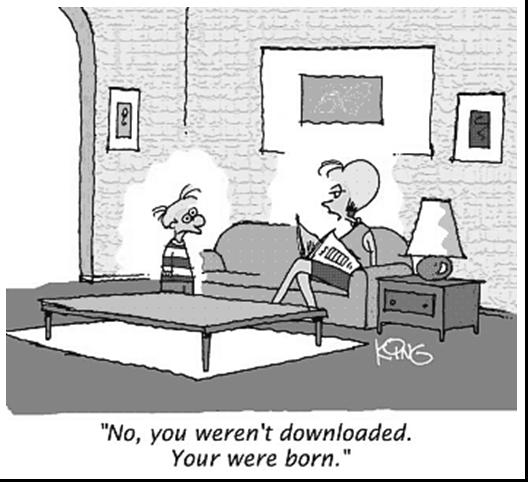
\includegraphics[width=.5\textwidth]{fig1.jpg}
\caption{A typical figure}
\label{fig:exampleFig1}
\end{figure}

\begin{figure}[ht]
\centering
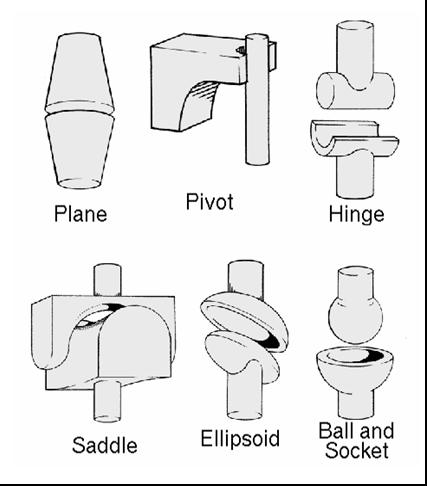
\includegraphics[width=.3\textwidth]{fig2.jpg}
\caption{This figure is an example of a figure caption taking more than one
  line and justified considering margins mentioned in Section~\ref{sec:figs}.}
\label{fig:exampleFig2}
\end{figure}

In tables, try to avoid the use of colored or shaded backgrounds, and avoid
thick, doubled, or unnecessary framing lines. When reporting empirical data,
do not use more decimal digits than warranted by their precision and
reproducibility. Table caption must be placed before the table (see Table 1)
and the font used must also be Helvetica, 10 point, boldface, with 6 points of
space before and after each caption.

\begin{table}[ht]
\centering
\caption{Variables to be considered on the evaluation of interaction
  techniques}
\label{tab:exTable1}
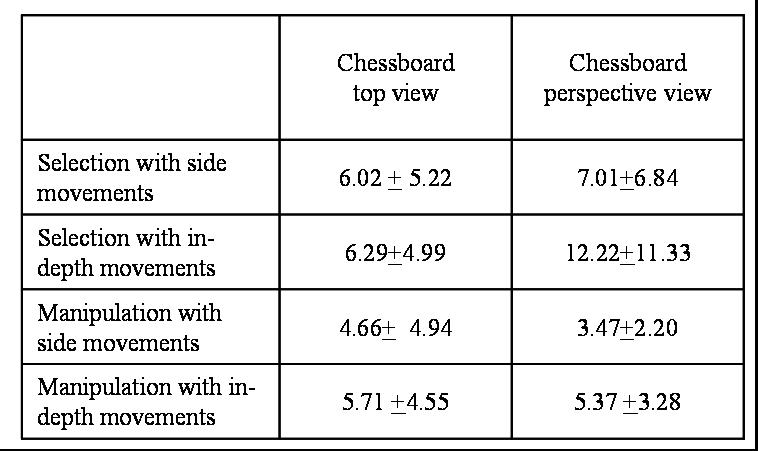
\includegraphics[width=.7\textwidth]{table.jpg}
\end{table}

\section{Images}

All images and illustrations should be in black-and-white, or gray tones,
excepting for the papers that will be electronically available (on CD-ROMs,
internet, etc.). The image resolution on paper should be about 600 dpi for
black-and-white images, and 150-300 dpi for grayscale images.  Do not include
images with excessive resolution, as they may take hours to print, without any
visible difference in the result.


\section{References}

Bibliographic references must be unambiguous and uniform.  We recommend giving
the author names references in brackets, e.g. \cite{knuth:84},
\cite{boulic:91}, \cite{smith:99}, \cite{Teste}.

The references must be listed using 12 point font size, with 6 points of space
before each reference. The first line of each reference should not be
indented, while the subsequent should be indented by 0.5 cm.

\end{comment}

\pagebreak

\bibliographystyle{sbc}
\bibliography{sbc-template}

\end{document}
